\documentclass[12pt,a4paper,openright,twoside]{report}


\usepackage[british]{babel}
\usepackage[utf8]{inputenc}


\usepackage{fancyhdr}
\usepackage{indentfirst}
\usepackage{graphicx}
\usepackage{newlfont}
\usepackage{xcolor}


\usepackage{amssymb}
\usepackage{amsmath}
\usepackage{latexsym}
\usepackage{amsthm}


\oddsidemargin=30pt 
\evensidemargin=20pt
\hyphenation{sil-la-ba-zio-ne pa-ren-te-si}
\pagestyle{fancy}\addtolength{\headwidth}{20pt}
\renewcommand{\chaptermark}[1]{\markboth{\thechapter.\ #1}{}}
\renewcommand{\sectionmark}[1]{\markright{\thesection \ #1}{}}
\rhead[\fancyplain{}{\bfseries\leftmark}]{\fancyplain{}{\bfseries\thepage}}
\cfoot{}
\linespread{1.3}

% Style theorem boxes

\theoremstyle{plain}
\newtheorem{prop}{Proposition}
\newtheorem{defin}{Definition}

\theoremstyle{definition}
\newtheorem{rem}{Remark}
\newtheorem{ex}{Example}


%%%%%%%%%%%%%%%%%%%%%%%%% DEDICATION %%%%%%%%%%%%%%%%%%%%%%%%%%%%%%%%%%%%%%%

\begin{document}

\begin{titlepage}
\thispagestyle{empty}                   
\topmargin=6.5cm                        
\raggedleft                             
\large                                  
                                       
\em                                     
To my beloved\\
Benedetta                   
\newpage                                

\clearpage{\pagestyle{empty}\cleardoublepage}
\end{titlepage}
\pagenumbering{roman}


            




%%%%%%%%%%%%%%%%%%%%%%% INTRODUCTION %%%%%%%%%%%%%%%%%%%%%%%%%%%%%%

\chapter*{Introduction}   
\addcontentsline{toc}{chapter}{Introduction}
\rhead[\fancyplain{}{\bfseries Introduction}]{\fancyplain{}{\bfseries\thepage}}\lhead[\fancyplain{}{\bfseries\thepage}]{\fancyplain{}{\bfseries Introduction}}




  \textcolor{blue}{Machine learning literature is exploding in size and complexity, but most solutions found are ad hoc, there is little communication between different subfields, and there is a large research debt. Category theory can solve these problems.  \cite{shieblerCategoryTheoryMachine2021}.}

  \textcolor{blue}{Talk about the origins of category theory and its "rise to power" as a common language that aims to unite different fields of knowledge.}
    
  \textcolor{blue}{Discuss the purpose of this work: a beginner-friendly survey of categorical approaches to neural networks, causal models, and interpretability.}





%%%%%%%%%%%%%%%%%%%%%%% ITALIAN TRANSLATION OF THE INTRODUCTION %%%%%%%%%%%%%%%%%%%%%%%%%%%%%%


\chapter*{Introduzione}
\addcontentsline{toc}{chapter}{Introduzione}
\rhead[\fancyplain{}{\bfseries Introduzione}]{\fancyplain{}{\bfseries\thepage}}\lhead[\fancyplain{}{\bfseries\thepage}]{\fancyplain{}{\bfseries Introduzione}}





  \textcolor{blue}{Traduzione italiana dell'introduzione.}







%\clearpage{\pagestyle{empty}\cleardoublepage}


%%%%%%%%%%%%%%%%%%%%%%%%%%%%% TABLE OF CONTENTS %%%%%%%%%%%%%%%%%%%%%%%%%%%%%%

\tableofcontents
\rhead[\fancyplain{}{\bfseries\leftmark}]{\fancyplain{}{\bfseries\thepage}} \lhead[\fancyplain{}{\bfseries\thepage}]{\fancyplain{}{\bfseries Table of Contents}}
%\clearpage{\pagestyle{empty}\cleardoublepage}

\listoffigures                         
%\clearpage{\pagestyle{empty}\cleardoublepage}


\listoftables                           
%\clearpage{\pagestyle{empty}\cleardoublepage}





%%%%%%%%%%%%%%%%%%%%%%%%% CATEGORICAL TOOLKIT %%%%%%%%%%%%%%%%%%%%%%%%%%%%%


\chapter{Categorical Toolkit}
\lhead[\fancyplain{}{\bfseries\thepage}]{\fancyplain{}{\bfseries\rightmark}}
\pagenumbering{arabic}



\textcolor{blue}{Brief introduction to category theory and the categorical toolkit used in the following sections. As each kind of category is introduced we shall also introduce appropriate string diagrams.}



  \section{Basics of Category Theory}


  \textcolor{blue}{Definition of category.}
  \textcolor{blue}{Definition of functor.}
  \textcolor{blue}{Definition of natural transformation.}
  \textcolor{blue}{Definition of 2-category.}


  \section{Various Families of Categories}

  \subsection{Monoidal Categories}

  \textcolor{blue}{Definition of monoidal category.}
  \textcolor{blue}{Definition of Cartesian category.}
  \textcolor{blue}{Definition of left-additive category.}
  \textcolor{blue}{Definition of Cartesian left-additive category.}

  \subsection{Differential Categories}

  \textcolor{blue}{Definition of Cartesian differential category.}
  \textcolor{blue}{Definition of reverse differential category.}
  \textcolor{blue}{Meaning of the associated differentiation operators.}
  \textcolor{blue}{Chain rules.}

  \textcolor{blue}{Reverse derivatives are more efficient and accurate than forward derivatives \cite{cockettReverseDerivativeCategories2019}.}



  \subsection{Lenses}

  \textcolor{blue}{Definition of lens. You can also mention the generic notion of optic here.}
  \textcolor{blue}{Analogy between the composition of lenses and the reverse chain rule.}
  \textcolor{blue}{C can be embedded in Lens(C).}



  \subsection{The Para Construction}

  \textcolor{blue}{Definition of M-Actegory.}
  \textcolor{blue}{Definition of Para.}
  \textcolor{blue}{Naturality of Para.}
  \textcolor{blue}{Embedding of Para(C) into Para(Lens(C)).}






  %\begin{figure}[h]
  %  \begin{center}                         
  %    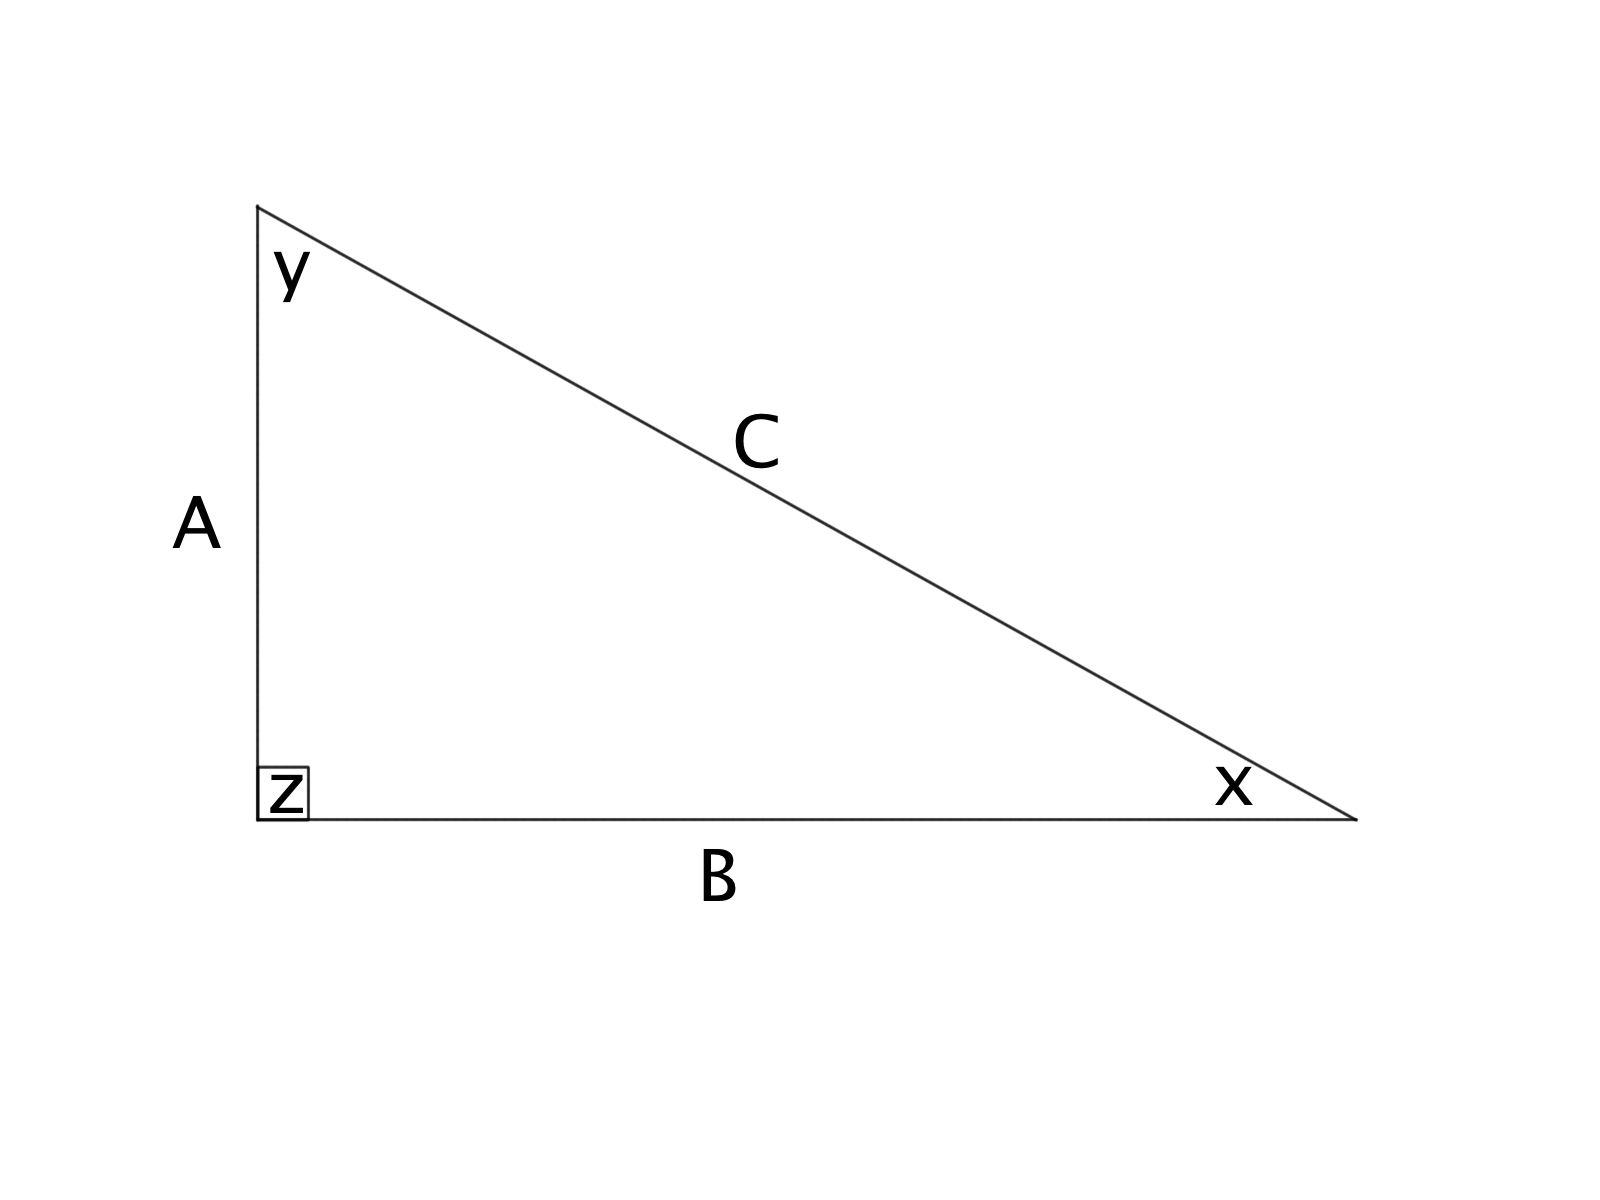
\includegraphics[width=5cm]{figures/triangle.jpg}
  %    \caption[Placeholder]{Placeholder figure.}\label{fig:first}
  %  \end{center}
  %\end{figure}

  %\begin{table}[h]                        
  %  \begin{center}                          
  %    \begin{tabular}{r|c|c}                  
  %      \hline \hline                           
  %      $(1,1)$ & $(1,2)$ & $(1,3)$\\           
  %      \hline                                  
  %      $(2,1)$ & $(2,2)$ & $(2,3)$\\           
  %      \hline                                  
  %      $(3,1)$ & $(3,2)$ & $(3,3)$\\
  %      \hline \hline                           
  %    \end{tabular}
  %    \caption[Placeholder Table]{Placeholder table.}\label{tab:uno}
  %  \end{center}
  %\end{table}



%%%%%%%%%%%%%%%%%%%%%%% CATEGORICAL APPROACHES TO NNS %%%%%%%%%%%%%%%%%%%%%%%%%%%


\chapter{Categorical Approaches to Neural Networks}
\lhead[\fancyplain{}{\bfseries\thepage}]{\fancyplain{}{\bfseries\rightmark}}




\textcolor{blue}{Brief summary of the chapter.}





\section{Neural Networks as Parametric Lenses}

\textcolor{blue}{Parametric lenses allow us to represent neural networks so that we can model both forward and backward propagation at the same time. This representation is compositional, and the learning iteration can also be represented \cite{cruttwellDeepLearningParametric}.}






\subsection{Neural Networks as Parametric Maps}





\subsection{Neural Networks as Parametric Lenses}





\subsection{Learning with Parametric Lenses}

\textcolor{blue}{Show that loss functions and optimizers can be represented as parametric lenses. Show that such components can be combined to actually model learning. Show that the learning iteration itself can be handled like this \cite{cruttwellDeepLearningParametric}.}

\textcolor{blue}{Parametric lenses can be successfully applied to software development \cite{cruttwellDeepLearningParametric}.}








%\clearpage{\pagestyle{empty}\cleardoublepage}

%%%%%%%%%%%%%%%%%%%%%%%%%%%%%% CONCLUSIONS %%%%%%%%%%%%%%%%%%%%%%%%%%%%%%%%%%%

\chapter*{Conclusions}
\rhead[\fancyplain{}{\bfseries
Conclusions}]{\fancyplain{}{\bfseries\thepage}}
\lhead[\fancyplain{}{\bfseries\thepage}]{\fancyplain{}{\bfseries Conclusions}}
\addcontentsline{toc}{chapter}{Conclusions} 










%%%%%%%%%%%%%%%%%%%%%%%%%%%%%%%%%%%%% BIBLIOGRAPHY %%%%%%%%%%%%%%%%%%%%%%%%%%%%%%

\bibliographystyle{apalike}
\bibliography{references}
\rhead[\fancyplain{}{\bfseries \:Bibliography}]{\fancyplain{}{\bfseries\thepage}} 
\addcontentsline{toc}{chapter}{Bibliography}



% \clearpage{\pagestyle{empty}\cleardoublepage}



%%%%%%%%%%%%%%%%%%%%%%%%%%%%%%%%%%%%%%% ACKNOWLEDGEMENTS %%%%%%%%%%%%%%%%%%%%%%%%%%%

\chapter*{Acknowledgements}

\thispagestyle{empty}

  Placeholder 



\end{document}
